\documentclass{article}

\usepackage{tikz}
\usetikzlibrary{matrix,backgrounds}
\usetikzlibrary{arrows,shapes,trees}
\usetikzlibrary{chains,shapes}

\usepackage{amsmath}


\newcommand{\chainlabel}[2]{\path [<-, draw, shorten >=10pt] (#1) |- node [at end] {#2} ++(-1,1);}



\begin{document}

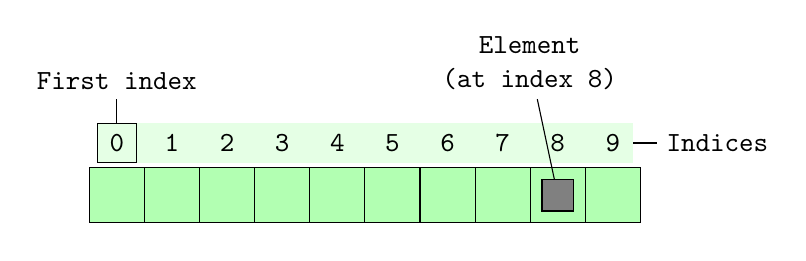
\begin{tikzpicture}[font=\ttfamily,
array/.style={matrix of nodes,nodes={draw, minimum size=7mm, fill=green!30},column sep=-\pgflinewidth, row sep=0.5mm, nodes in empty cells,
row 1/.style={nodes={draw=none, fill=none, minimum size=5mm}},
row 1 column 1/.style={nodes={draw}}}]

\matrix[array] (array) {
0 & 1 & 2 & 3 & 4 & 5 & 6 & 7 & 8 & 9\\
  &   &   &   &   &   &   &   &   &  \\};
\node[draw, fill=gray, minimum size=4mm] at (array-2-9) (box) {};

\begin{scope}[on background layer]
\fill[green!10] (array-1-1.north west) rectangle (array-1-10.south east);
\end{scope}

\draw (array-1-1.north)--++(90:3mm) node [above] (first) {First index};
\draw (array-1-10.east)--++(0:3mm) node [right]{Indices};
\node [align=center, anchor=south] at (array-2-9.north west|-first.south) (8) {Element\\ (at index 8)};
\draw (8)--(box);
%
\end{tikzpicture}
\\
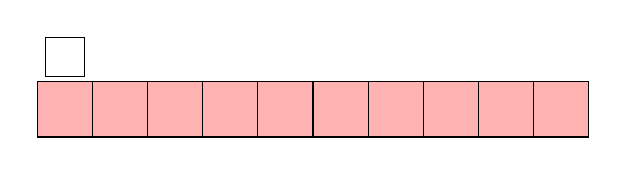
\begin{tikzpicture}[font=\ttfamily,
array/.style={matrix of nodes,nodes={draw, minimum size=7mm, fill=red!30},column sep=-\pgflinewidth, row sep=0.5mm, nodes in empty cells,
row 1/.style={nodes={draw=none, fill=none, minimum size=5mm}},
row 1 column 1/.style={nodes={draw}}}]

\matrix[array] (array) {
 &  &  &  &  &  &  &  &  & \\
 &   &   &   &   &   &   &   &   &  \\};
%
\end{tikzpicture}
\\
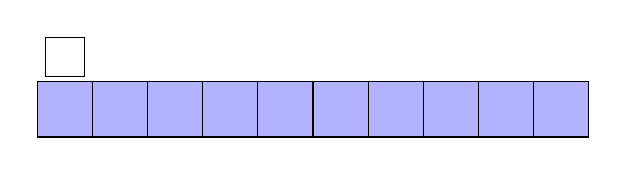
\begin{tikzpicture}[font=\ttfamily,
array/.style={matrix of nodes,nodes={draw, minimum size=7mm, fill=blue!30},column sep=-\pgflinewidth, row sep=0.5mm, nodes in empty cells,
row 1/.style={nodes={draw=none, fill=none, minimum size=5mm}},
row 1 column 1/.style={nodes={draw}}}]

\matrix[array] (array) {
 &  &  &  &  &  &  &  &  & \\
 &   &   &   &   &   &   &   &   &  \\};
%
\end{tikzpicture}






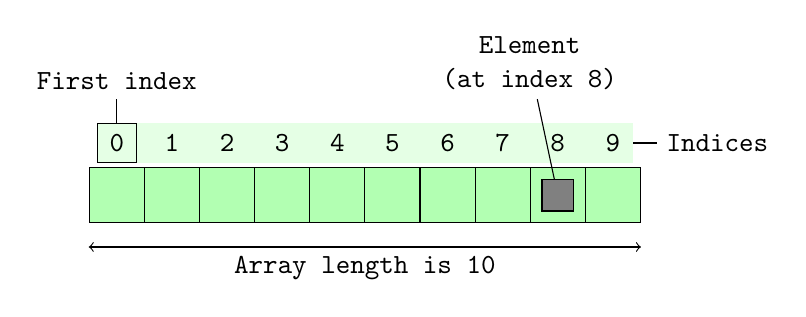
\begin{tikzpicture}[font=\ttfamily,
array/.style={matrix of nodes,nodes={draw, minimum size=7mm, fill=green!30},column sep=-\pgflinewidth, row sep=0.5mm, nodes in empty cells,
row 1/.style={nodes={draw=none, fill=none, minimum size=5mm}},
row 1 column 1/.style={nodes={draw}}}]

\matrix[array] (array) {
0 & 1 & 2 & 3 & 4 & 5 & 6 & 7 & 8 & 9\\
  &   &   &   &   &   &   &   &   &  \\};
\node[draw, fill=gray, minimum size=4mm] at (array-2-9) (box) {};

\begin{scope}[on background layer]
\fill[green!10] (array-1-1.north west) rectangle (array-1-10.south east);
\end{scope}

\draw[<->]([yshift=-3mm]array-2-1.south west) -- node[below] {Array length is 10} ([yshift=-3mm]array-2-10.south east);

\draw (array-1-1.north)--++(90:3mm) node [above] (first) {First index};
\draw (array-1-10.east)--++(0:3mm) node [right]{Indices};
\node [align=center, anchor=south] at (array-2-9.north west|-first.south) (8) {Element\\ (at index 8)};
\draw (8)--(box);
%
\end{tikzpicture}



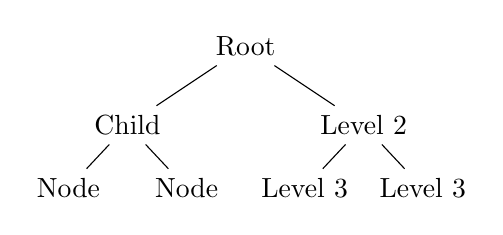
\begin{tikzpicture}[level distance=1.3cm,
   level 1/.style={sibling distance=3cm, level distance=1cm},
   level 2/.style={sibling distance=1.5cm, level distance=0.8cm}]
\node {Root}
   child {node {Child}
   child {node {Node}}
   child {node {Node}}
}
child {node {Level 2}
   child {node {Level 3}}
   child {node {Level 3}}
};
\end{tikzpicture}






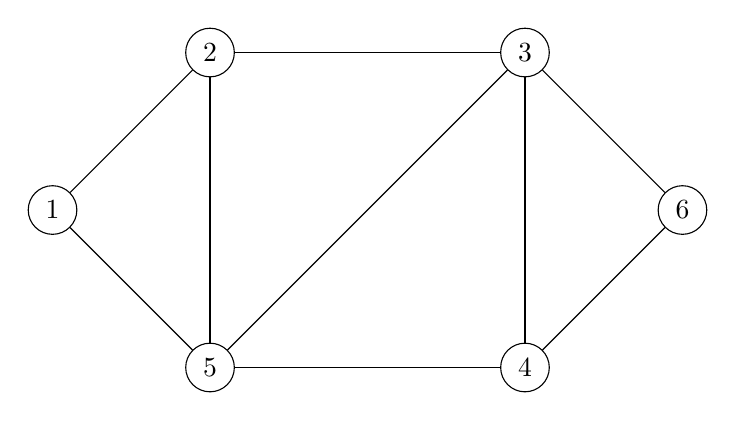
\begin{tikzpicture}
     \tikzstyle{node_style} = [circle,draw=black]
     \tikzstyle{edge_style} = [draw=black]
     \node[node_style] (v1) at (-2,2) {2};
     \node[node_style] (v2) at (2,2) {3};
     \node[node_style] (v3) at (4,0) {6};
     \node[node_style] (v4) at (2,-2) {4};
     \node[node_style] (v5) at (-2,-2) {5};
     \node[node_style] (v6) at (-4,0) {1};
     \draw[edge_style]  (v1) edge (v2);
     \draw[edge_style]  (v2) edge (v3);
     \draw[edge_style]  (v3) edge (v4);
     \draw[edge_style]  (v4) edge (v5);
     \draw[edge_style]  (v5) edge (v6);
     \draw[edge_style]  (v6) edge (v1);
     \draw[edge_style]  (v5) edge (v1);
     \draw[edge_style]  (v5) edge (v2);
     \draw[edge_style]  (v4) edge (v2);
\end{tikzpicture}






\begin{tikzpicture}[draw, minimum width=1cm, minimum height=0.5cm]
    \node[draw] (in) at (-1,2) {};
    \node[draw] (out) at (1,-2) {};
    \matrix (queue)[matrix of nodes, nodes={draw, nodes={draw}}, nodes in empty cells]
    {
       \\ \\ \\ \\
    };

    \draw[-latex] (0.25,-1) .. controls (0.25,-1.25) and (1,-1.25) .. (out.north);
    \draw[-latex] (in.south) .. controls (-1, 1.5) and (-0.25,1.5) .. (-0.25,1);
\end{tikzpicture}









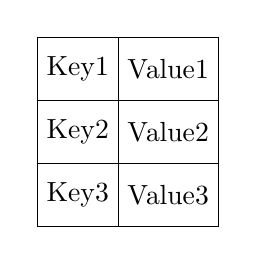
\begin{tikzpicture} [nodes={minimum width=0.8cm, minimum height=0.8cm},
         row sep=-\pgflinewidth, column sep=-\pgflinewidth]
   \matrix (hash)[matrix of nodes, nodes={draw, anchor=center}]
         {
       Key1 & Value1 \\
       Key2 & Value2 \\
       Key3 & Value3 \\
    };
\end{tikzpicture}



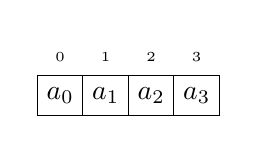
\begin{tikzpicture} [nodes in empty cells,
      nodes={minimum width=0.5cm, minimum height=0.5cm},
      row sep=-\pgflinewidth, column sep=-\pgflinewidth]
      border/.style={draw}
    
      \matrix(vector)[matrix of nodes,
          row 1/.style={nodes={draw=none, minimum width=0.3cm}},
          nodes={draw}]
      {
          \tiny{0} & \tiny{1} & \tiny{2} & \tiny{3}\\
          $a_{0}$ & $a_{1}$ & $a_{2}$ & $a_{3}$\\
      };
\end{tikzpicture}




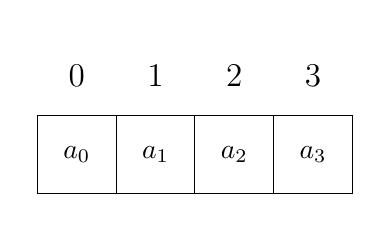
\begin{tikzpicture} [nodes in empty cells,
      nodes={minimum width=1cm, minimum height=1cm},
      row sep=-\pgflinewidth, column sep=-\pgflinewidth]
      border/.style={draw}
    
      \matrix(vector)[matrix of nodes,
          row 1/.style={nodes={draw=none, minimum width=0.3cm}},
          nodes={draw}]
      {
      	   
          \large{0} & \large{1} & \large{2} & \large{3} \\
          $a_{0}$ & $a_{1}$ & $a_{2}$ & $a_{3}$ \\
      };
\end{tikzpicture}







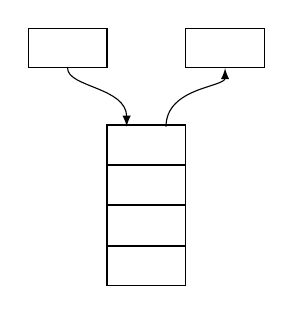
\begin{tikzpicture}[draw, minimum width=1cm, minimum height=0.5cm]
    \node[draw] (in) at (-1,2) {};
    \node[draw] (out) at (1,2) {};
    \matrix (queue)[matrix of nodes, nodes={draw, nodes={draw}}, nodes in empty cells]
    {
       \\ \\ \\ \\
    };

    \draw[-latex] (0.25,1) .. controls (0.25,1.5) and (1,1.5) .. (out.south);
    \draw[-latex] (in.south) .. controls (-1, 1.5) and (-0.25,1.5) .. (-0.25,1);
\end{tikzpicture}








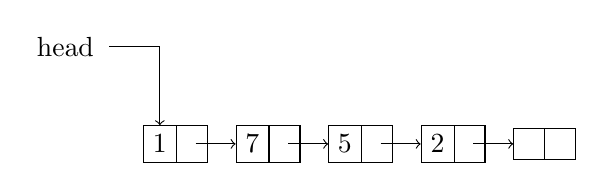
\begin{tikzpicture}[every node/.style={rectangle split, rectangle split parts=2, rectangle split horizontal}, node distance=1em, start chain, 
 every join/.style={->, shorten <=-4.5pt}]

 \node[draw, on chain, join] { 1  };
 \node[draw, on chain, join] { 7  };
 \node[draw, on chain, join] { 5  };
 \node[draw, on chain, join] { 2  };
 \node[draw, on chain, join] {};
\chainlabel{chain-1.one north}{head};
\end{tikzpicture}  

{
.
\\
\\
}

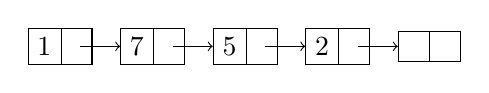
\begin{tikzpicture}[every node/.style={rectangle split, rectangle split parts=2, rectangle split horizontal}, node distance=1em, start chain, 
 every join/.style={->, shorten <=-4.5pt}]

 \node[draw, on chain, join] { 1  };
 \node[draw, on chain, join] { 7  };
 \node[draw, on chain, join] { 5  };
 \node[draw, on chain, join] { 2  };
 \node[draw, on chain, join] {};
%\chainlabel{chain-1.one north}{head};
\end{tikzpicture}  




\end{document}